\documentclass[10pt,a4paper]{beamer}
\usepackage[utf8]{inputenc}
\usepackage[francais]{babel}
\usepackage[T1]{fontenc}
\usepackage{amsmath}

\usepackage{amsfonts}
\usepackage{amssymb}

\usetheme[secheader]{Boadilla}
%\usepackage{caption}


\usepackage[usenames,dvipsnames]{pstricks}
%\usepackage{epsfig}
%\usepackage{pst-grad} % For gradients
%\usepackage{pst-plot} % For axes

%\usepackage{movie15}

\graphicspath{{figures/}}


\title[IRTG Presentation]{PGD for low frequency dynamics problems involving localized non-linearities}
\author[Pierre NARGIL]{Pierre NARGIL\\Supervisors : 
\large{\\François LOUF\\Pierre-Alain BOUCARD} }
\institute{LMT Cachan}
\date{Wednesday 7th May 2014}


\begin{document}

\begin{frame}
	\titlepage
\end{frame}

\section{MECASIF Project}

\begin{frame}{Project origin}
	\vspace{-0.3cm}
	\begin{center}
		\begin{figure}
		\begin{minipage}{0.70\linewidth}
				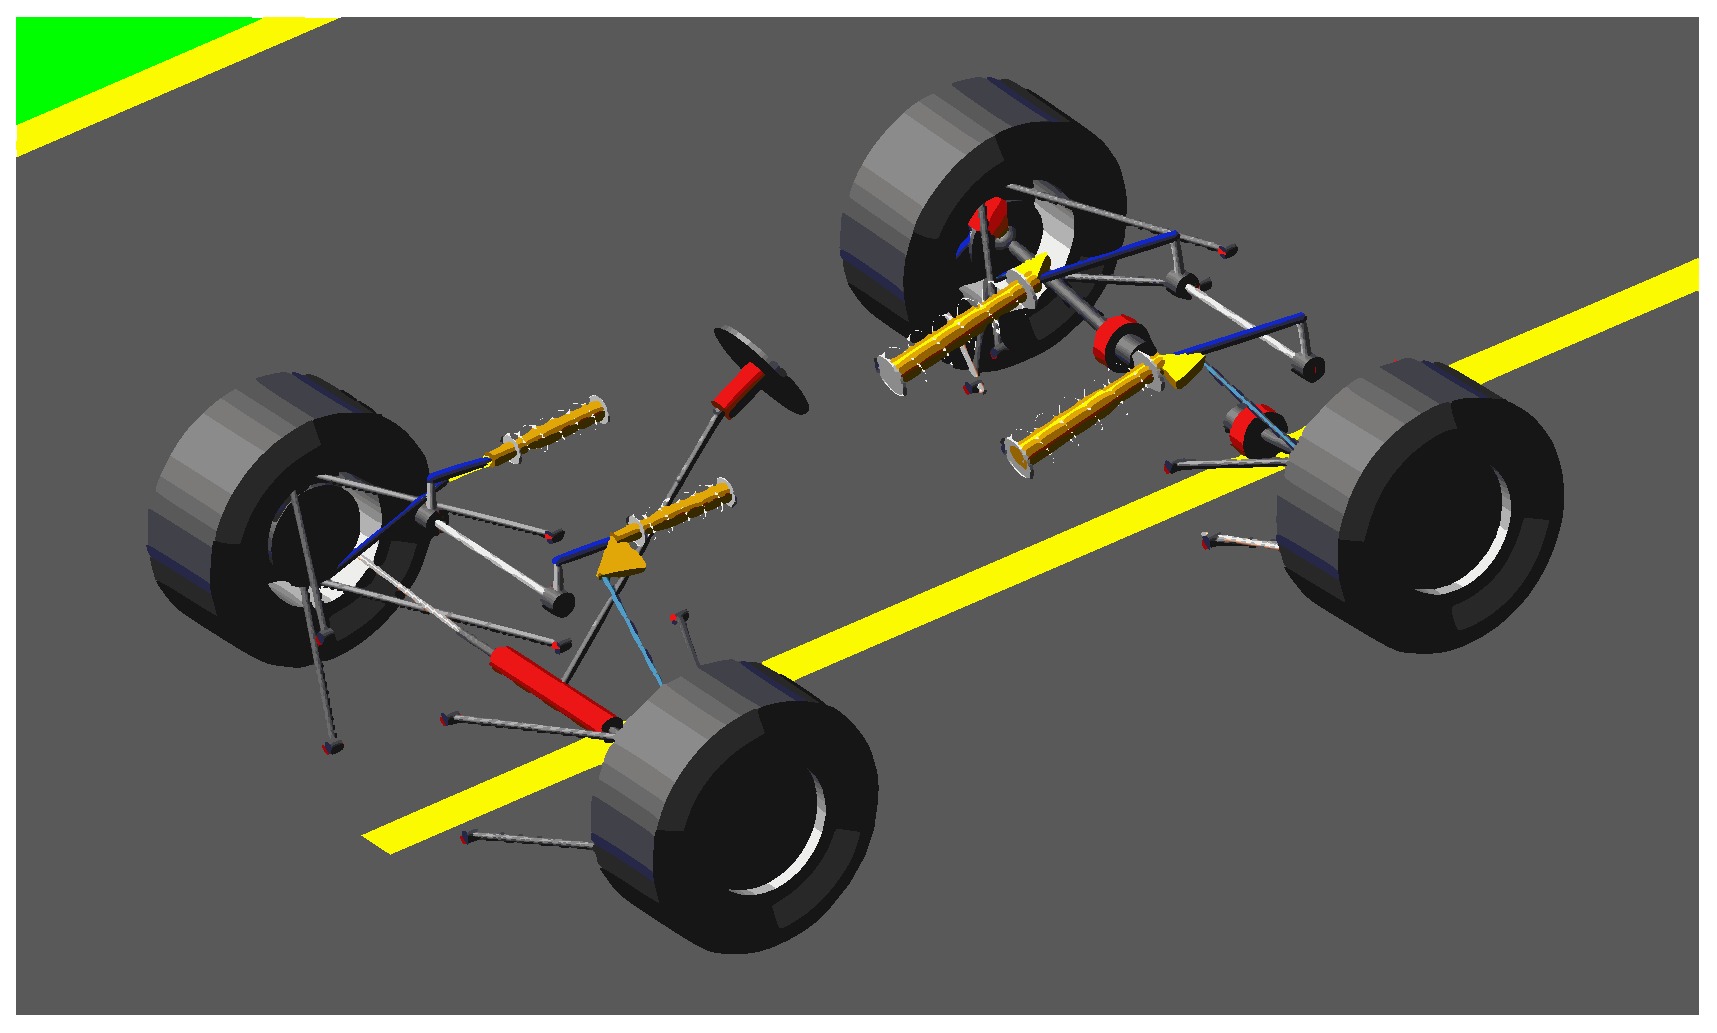
\includegraphics[width=1\linewidth]{roulage.eps}
				\caption{Industrial problem}
			\end{minipage}
		\end{figure}
	\end{center}
	\vspace{-0.5cm}
	\begin{itemize}
		\item Calculation time
		\item Set of parameters
		\item Non-linearity
	\end{itemize}
\end{frame}

\section*{}

\begin{frame}{Presentation plan}
	\begin{block}{}
		%\vfill
			\hspace{1cm}
			\begin{minipage}[l][0.650\textheight]{0.30\linewidth}
				\setcounter{tocdepth}{2}
				\tableofcontents
			\end{minipage}
			\vspace{0.5cm}
	\end{block}
\end{frame}

\section{Model Order Reduction}

\begin{frame}{Model order reduction}
	Reducing calculation time by reducing the dimension of the problem
	\begin{block}{Stakes of time saving}
	{
	\begin{itemize}
	\item Reducing the developement cost
	\item Optimisation / Creation of probabilistic models
	\item Solving of problems reaching calculating machine's limits
	\end{itemize}
	}
	\end{block}
	
	Reduced order modeling : Solving projected problems\\
	How to obtain the basis to project on :
	\begin{block}{Reduction methods}
	{
	\begin{itemize}
	\item POD - Proper Orthogonal Decomposition [A. Chatterjee - 2000]
	\item PGD - Proper Generalized Decomposition [P. Ladevèze - 1989]
	\end{itemize}
	}
	\end{block}
	
	% La réduction de modèles apporte une réduction du temps de calcul. 
	% En réduisant la dimension du problème, 
	%	on diminue le nombre d'opérations nécessaires à sa résolution.
	%
	% La réduction de modèles consiste à résoudre un problème 
	%	après l'avoir projeté sur une base de dimension inférieure
	%	à celle de la base d'origine.
	% Il existe différentes méthodes pour obtenir ces bases.


\end{frame}


\section{Different methods}

\begin{frame}{Presentation plan}
\addtocounter{framenumber}{-1}
	\begin{block}{}
		%\vfill
			\hspace{1cm}
			\begin{minipage}[l][0.650\textheight]{0.30\linewidth}
				\setcounter{tocdepth}{2}
				\tableofcontents[currentsection] 
			\end{minipage}
			\vspace{0.5cm}
	\end{block}
\end{frame}


\begin{frame}{Different methods}
	
	\begin{figure}
   \begin{minipage}{0.47\linewidth}
		\begin{exampleblock}{POD}
		\vbox to .7\textheight{%
			\begin{itemize}
			\item a posteriori
			\item give modes in:
				\begin{itemize}
				\item space
				\item time
				\end{itemize}
			\end{itemize}
			\vspace{0.395cm}
			\begin{itemize}
			\item Principle :
			\end{itemize}
			Projection on a basis of modes exctracted from truncated SVD
			%	À partir de la solution d'un problème à laquelle 
			%	on applique une SVD, on trouve les modes principaux 
			%	associés aux valeurs singulières les plus élevées.
			\vfill
		}
		\end{exampleblock}
   \end{minipage}\hfill
   \begin{minipage}{0.47\linewidth}
		\begin{alertblock}{PGD}
		\vbox to .7\textheight{%
			\begin{itemize}
			\item modes calculation "on the fly"
				\item give modes in :
					\begin{itemize}
					\item space
					\item time
					\item parameter
					\end{itemize}
			\end{itemize}
			\begin{itemize}
			\item Principle :
			\end{itemize}
			Modes calculated using an iterative method (fixed point)
			 at the same time as the resolution.	
			%	À partir des données d'un problème on calcule les modes 
			%	"à la volée" par une méthode de point fixe en résolvant.
			\vfill
		}
		\end{alertblock}
   \end{minipage}
   \hfill
\end{figure}

\end{frame}

\subsection{POD}

\begin{frame}{Proper Orthogonal Decomposition}
	
	\begin{exampleblock}{A dynamic problem is solved on the system, and the SVD gives :}
	$ \displaystyle U(X,t) = \sum_{k=1}^{dim} V_{Sk}~f_k(X) g_k(t)$\\
	\end{exampleblock}
		
	\begin{exampleblock}{The basis is obtained by truncating the result}
	The $n$ modes $f_k(X)$ associated to the highest 
	singular values are chose to make the reduced basis.\\
	The SVD guarantees the best truncated basis such as :
	$ \displaystyle U(X,t) - U_n(X,t) = U(X,t) - \sum_{k=1}^{n} V_{Sk}~ f_k(X) g_k(t)$\\
	is minimal for a fixed $n$ (in Frobenius norm).\\
	These couples are the more representative of the studied response.
	\end{exampleblock}
	\vspace{-0.3cm}
	\begin{figure}
	   \begin{minipage}{0.22\linewidth}
			\begin{exampleblock}{}
				\centering		
				Solving (Snapshot)
				%\vspace{0.22cm}
			\end{exampleblock}
	   \end{minipage}\hfill
	   \begin{minipage}{0.03\linewidth}
			\vspace{0.220cm}
	   		$\rightarrow$
	   \end{minipage}\hfill
	   \begin{minipage}{0.22\linewidth}
			\begin{exampleblock}{}
				\centering		
				%\vspace{0.210cm}
				Get the reduced basis
				%\vspace{0.22cm}
			\end{exampleblock}
	   \end{minipage}\hfill
	   \begin{minipage}{0.03\linewidth}
			\vspace{0.220cm}
	   		$\rightarrow$
	   \end{minipage}\hfill
	   \begin{minipage}{0.22\linewidth}
			\begin{exampleblock}{}
				\centering		
				Projection on the reduced basis
			\end{exampleblock}
	   \end{minipage}\hfill
	   \begin{minipage}{0.03\linewidth}
			\vspace{0.220cm}
	   		$\rightarrow$
	   \end{minipage}\hfill
	   \begin{minipage}{0.22\linewidth}
			\begin{exampleblock}{}
				\centering		
				\vspace{0.21cm}
				Solving
				\vspace{0.22cm}
			\end{exampleblock}
	   \end{minipage}
	\end{figure}
		
\end{frame}

\setbeamertemplate{caption}{\insertcaption}
%\setbeamertemplate{caption}{skip=0pt}

\begin{frame}{Picture Compression - Different number of singular values} 
	%
	\begin{figure}
		\begin{minipage}{0.24\linewidth}
			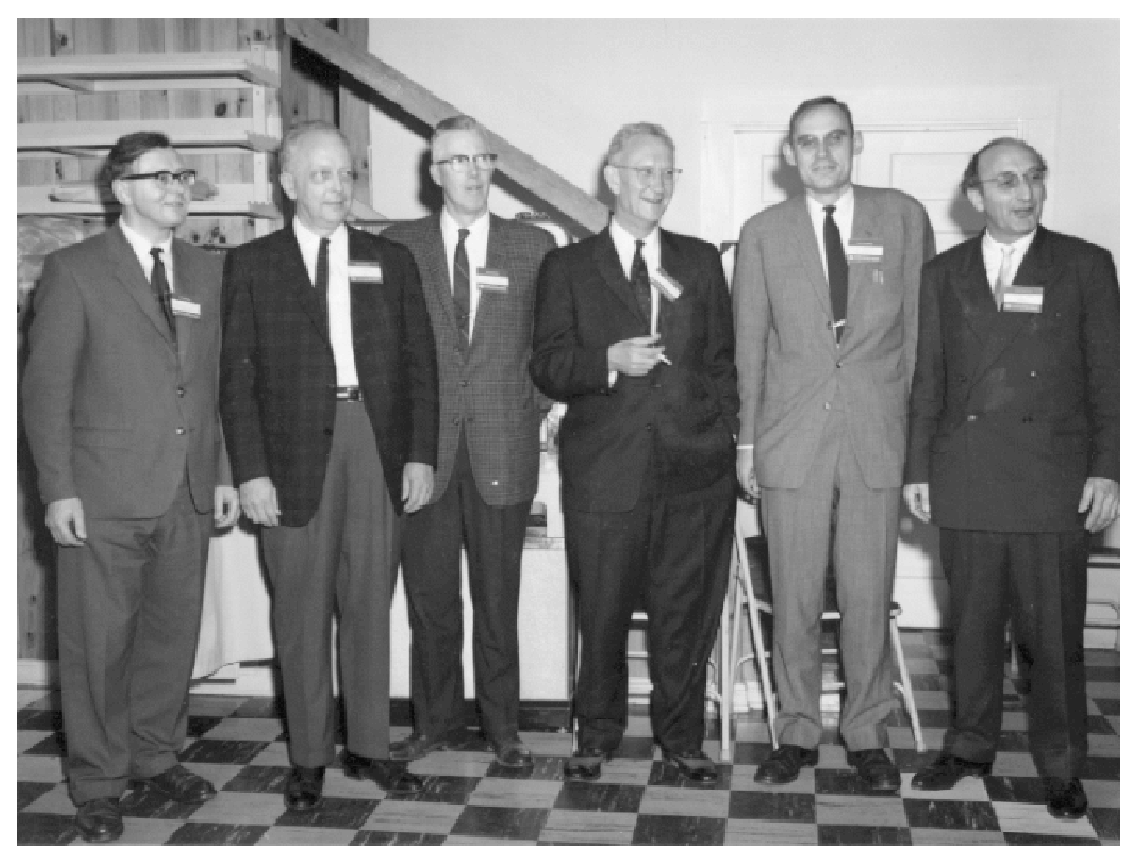
\includegraphics[width=1\linewidth]{SVD/Image.originale.eps}
				\caption{Original}
		\end{minipage}
		\begin{minipage}{0.24\linewidth}
			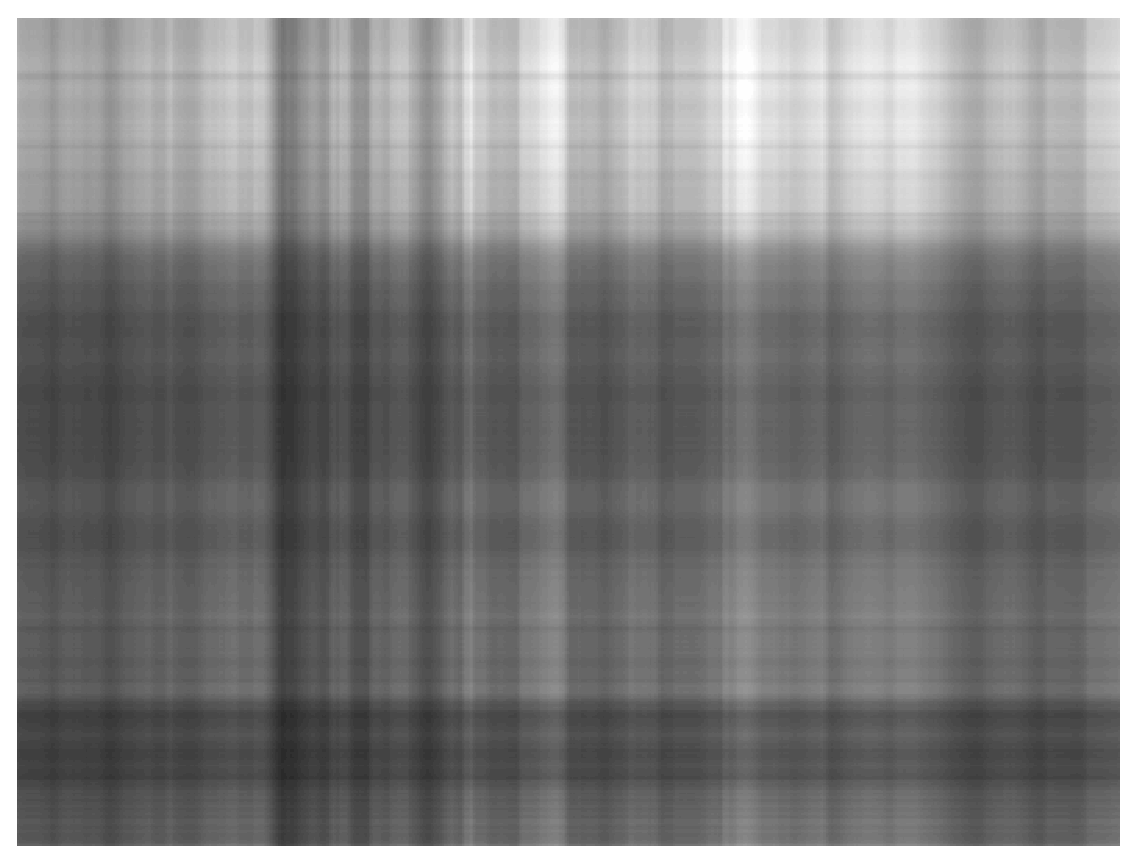
\includegraphics[width=1\linewidth]{SVD/SVD.Tronquee.1.eps}
				\caption{1 value}
		\end{minipage}
		\begin{minipage}{0.24\linewidth}
			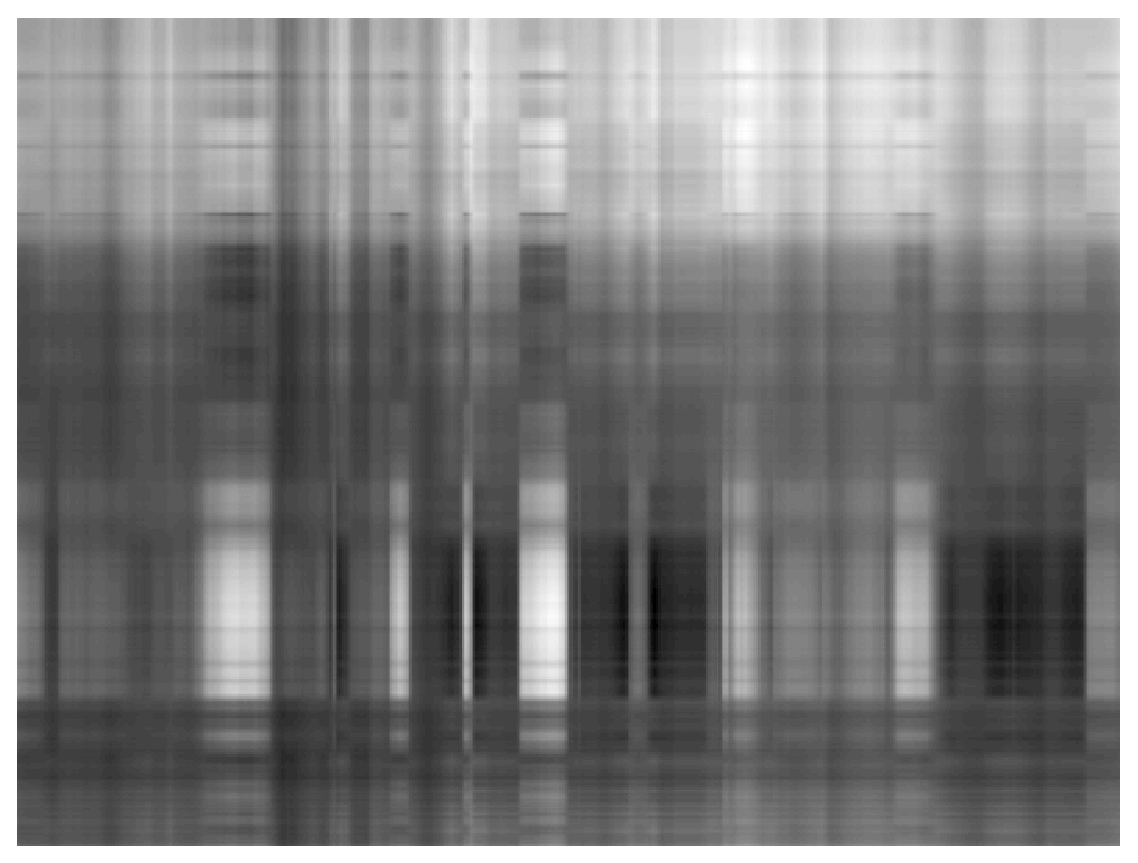
\includegraphics[width=1\linewidth]{SVD/SVD.Tronquee.2.eps}
				\caption{2 values}
		\end{minipage}
		\begin{minipage}{0.24\linewidth}
			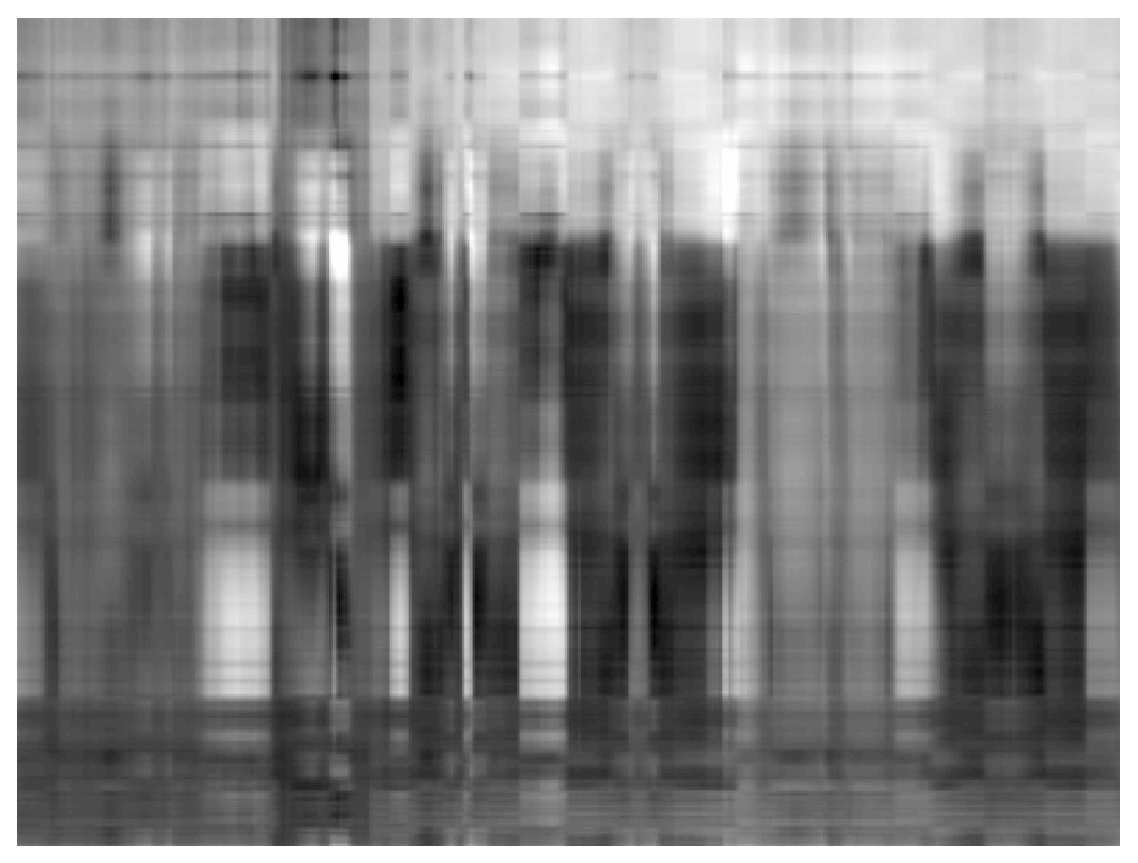
\includegraphics[width=1\linewidth]{SVD/SVD.Tronquee.4.eps}
				\caption{4 values}
		\end{minipage}
	\end{figure}
	\vspace{-0.4cm}
	
	\begin{figure}
	%\captionsetup[figure]{skip=2pt}
		\begin{minipage}{0.24\linewidth}
			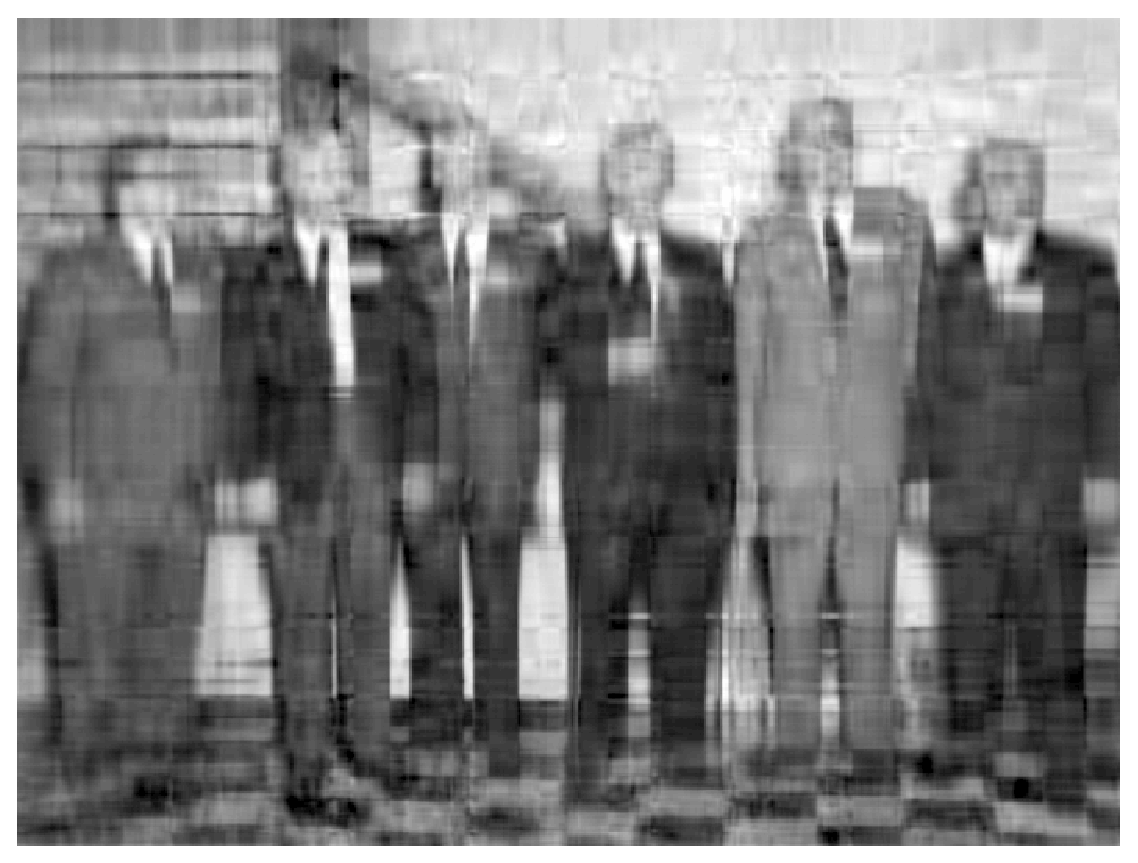
\includegraphics[width=1\linewidth]{SVD/SVD.Tronquee.16.eps}
				\caption{16 values}
		\end{minipage}
		\begin{minipage}{0.24\linewidth}
			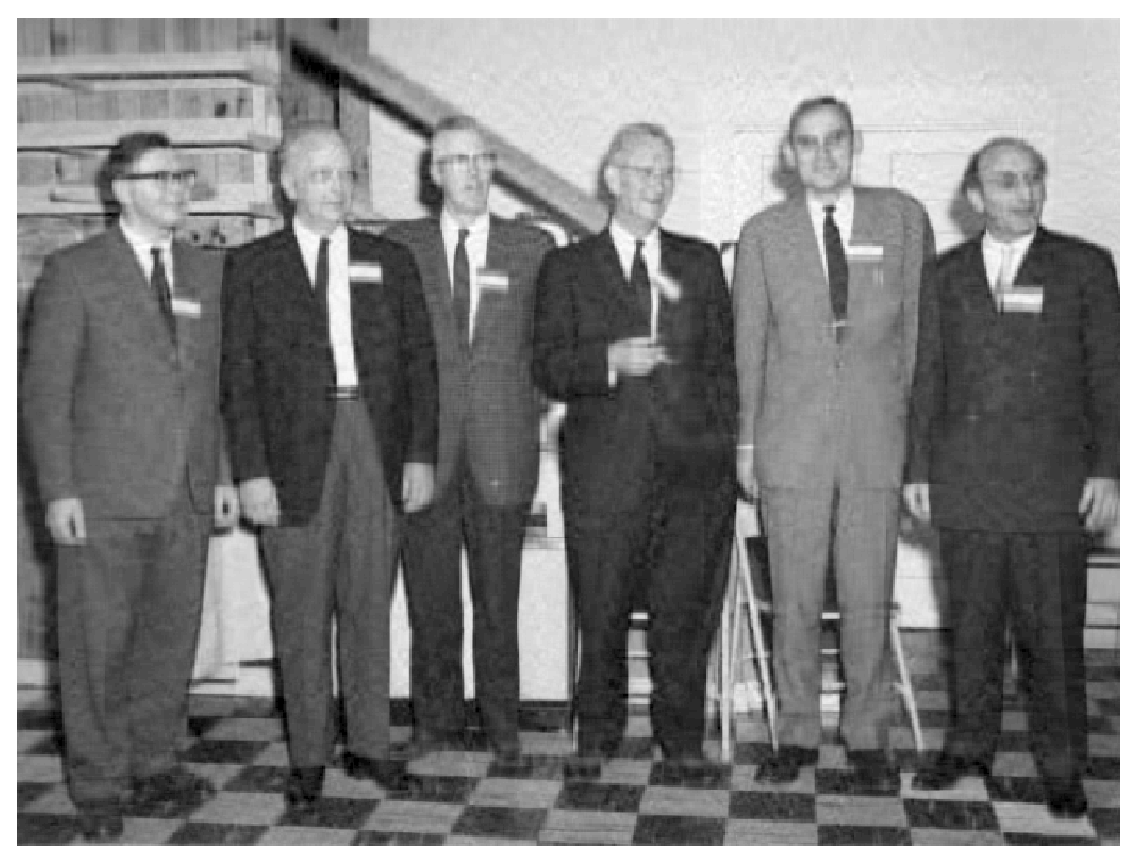
\includegraphics[width=1\linewidth]{SVD/SVD.Tronquee.64.eps}
				\caption{64 values}
		\end{minipage}
		\begin{minipage}{0.24\linewidth}
			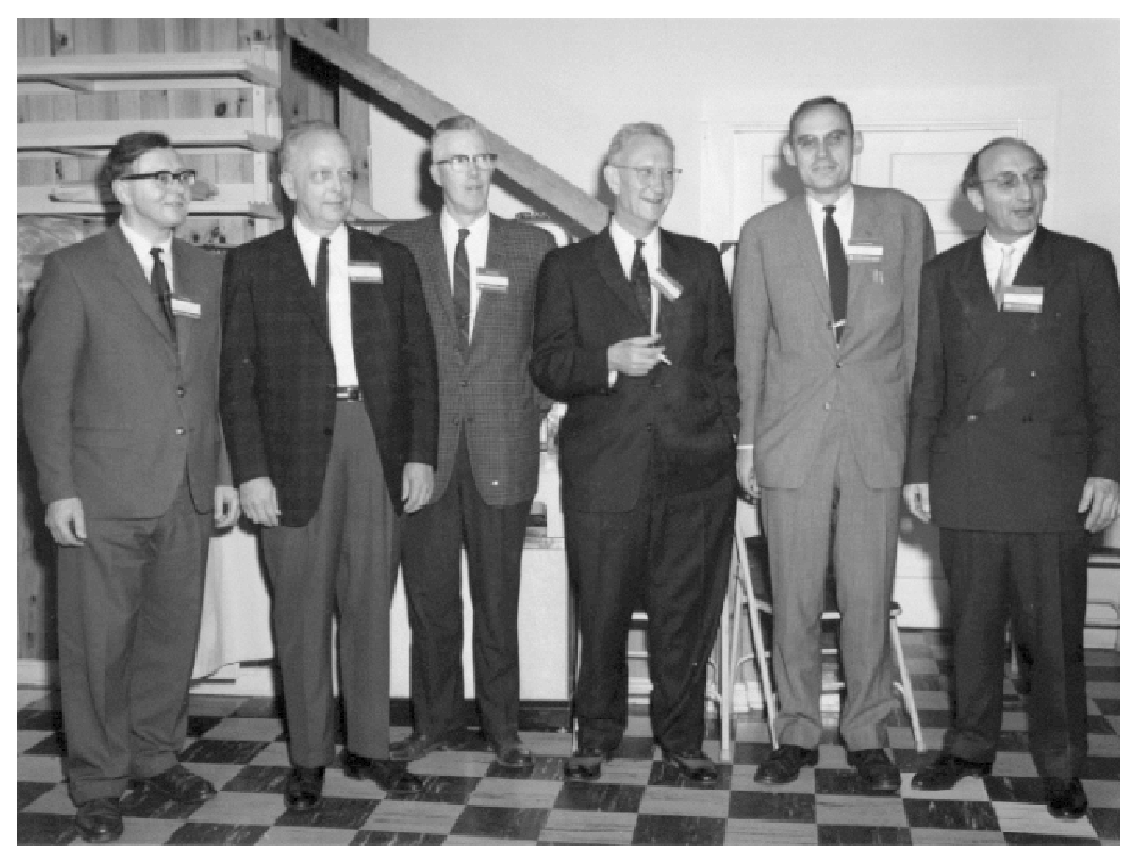
\includegraphics[width=1\linewidth]{SVD/SVD.Tronquee.256.eps}
				\caption{256 values}
		\end{minipage}
		\begin{minipage}{0.24\linewidth}
			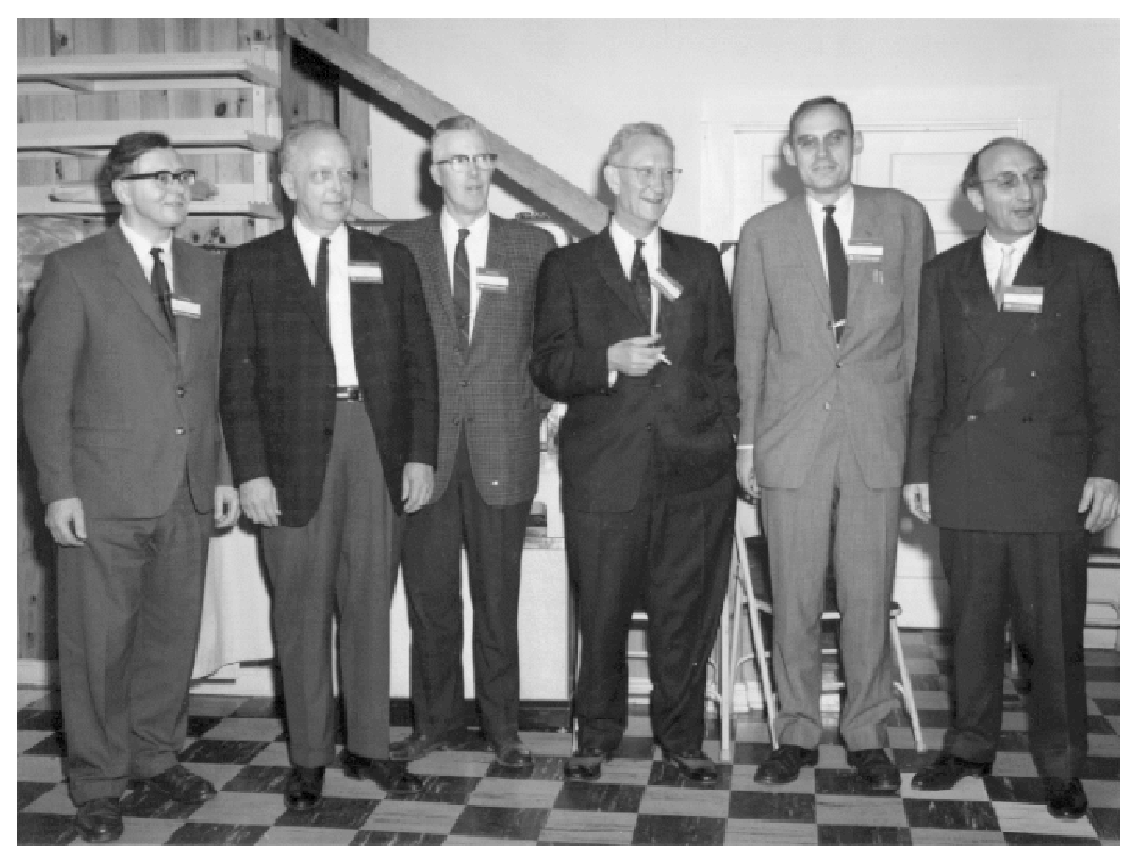
\includegraphics[width=1\linewidth]{SVD/SVD.Total.eps}
				\caption{Total (480)}
		\end{minipage}
	\end{figure}
\end{frame}

\setbeamertemplate{caption}[default]

\subsection{PGD}

\begin{frame}{Proper Generalized Decomposition}
	
	\begin{alertblock}{Approximation using separable variables}
	$ \displaystyle U_n(X,t,\lambda) = \sum_{k=1}^n 
											f_k(X) g_k(t) h_k(\lambda)$
	\end{alertblock}
	\vspace{-0.1cm}
	\begin{alertblock}{The variational formulation gives a problem for each type of function}
	$ f_k = F (U_{k-1},g_k,h_k)~,~~~~~
	 g_k = G (U_{k-1},f_k,h_k)~,~~~~~
	 h_k = H (U_{k-1},f_k,g_k)$
	\end{alertblock}
	\vspace{-0.4cm}
	\begin{figure}[t]
	   \begin{minipage}[l]{0.40\linewidth}
			\begin{alertblock}{Algorithm}
			%\vbox to .3\textheight
			\end{alertblock}
	   \end{minipage}\hfill
	   \begin{minipage}{0.54\linewidth}
			\begin{alertblock}{}
			%\vbox to .7\textheight
			\end{alertblock}
	   \end{minipage}
	\end{figure}
	\vfill
	
\end{frame}

\section{A few results}

\begin{frame}{Presentation plan}
\addtocounter{framenumber}{-1}
	\begin{block}{}
		%\vfill
			\hspace{1cm}
			\begin{minipage}[l][0.650\textheight]{0.30\linewidth}
				\setcounter{tocdepth}{2}
				\tableofcontents[currentsection] 
			\end{minipage}
			\vspace{0.5cm}
	\end{block}
\end{frame}

\subsection{Error}

\begin{frame}{Error indicators}
%	\begin{equation}
%		e_ {Amp} = \left|\frac{max(s_ {Ref}) - min(s_ {Ref}) 
%							- \big[ max(s_ {Cal}) - min(s_ {Cal}) \big] }
%		{max(s_ {Ref}) - min(s_ {Ref})} \right|
%	\end{equation}
	
	\begin{equation}
		e_ {Max} = \left|\frac{ max(s_ {Ref} - s_ {Cal}) }
		{max(s_ {Ref}) - min(s_ {Ref})} \right|
	\end{equation}
	
	\begin{figure}
		\begin{minipage}{0.47\linewidth}
			\includegraphics[width=1\linewidth]{Calcul100M.POD.tikz.eps}
			\caption{\centering Evolution of error indicators for a POD Solution}		
		\end{minipage}
		 \hspace{0.5cm}
		\begin{minipage}{0.47\linewidth}
			\includegraphics[width=1\linewidth]{Calcul100M.PGD.tikz.eps}
			\caption{\centering Evolution of error indicators for a PGD Solution}		
		\end{minipage}
	\end{figure}
	
\end{frame}

\subsection{MAC}

\begin{frame}{MAC Analysis 
	$\frac{\left(\boldsymbol{\varphi_i.\psi_j}\right)^2}{\boldsymbol{\varphi_i.\varphi_i \times \psi_j.\psi_j}}$} 
	\begin{figure}
		\begin{minipage}{0.47\linewidth}
			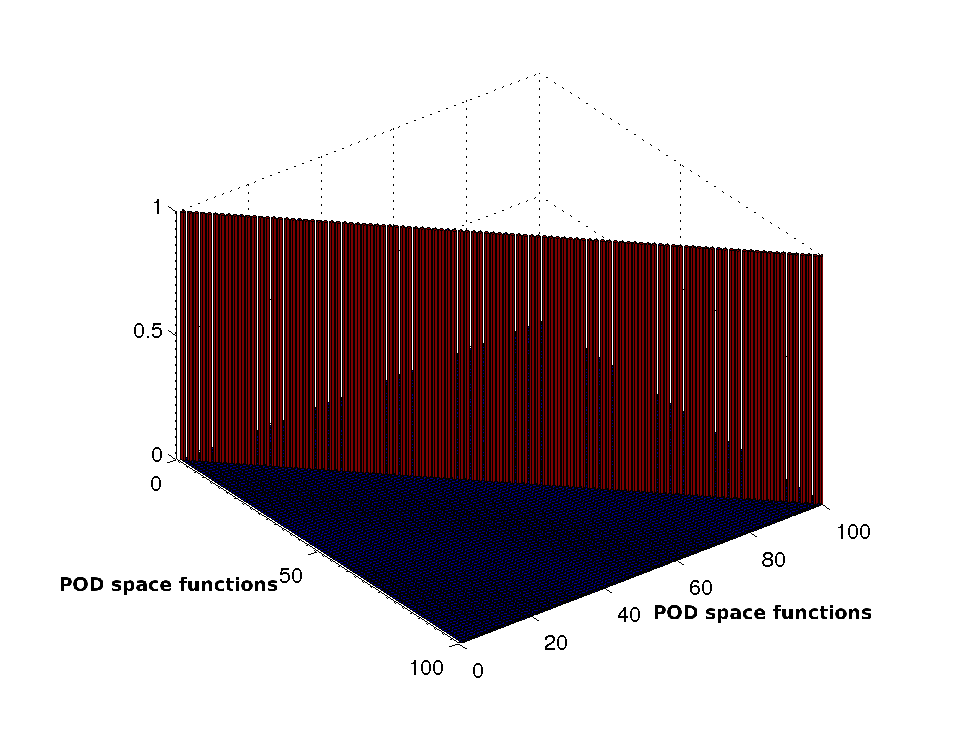
\includegraphics[width=1\linewidth]{MAC-POD2.eps}
			\caption{\centering POD space functions}		
		\end{minipage}
		 \hspace{0.5cm}
		\begin{minipage}{0.47\linewidth}
			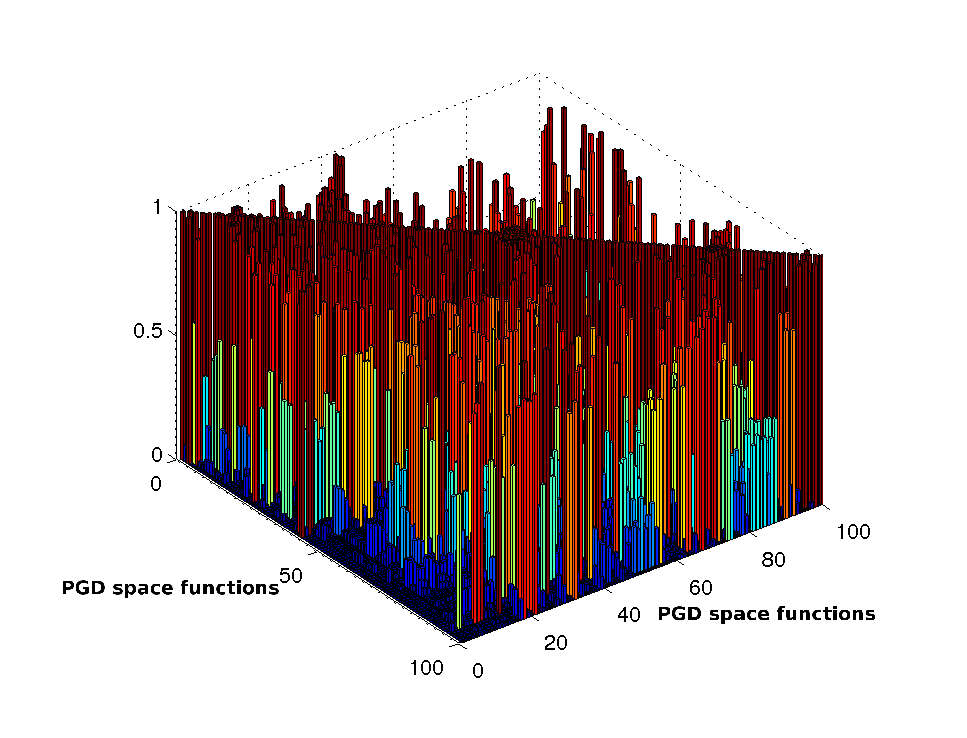
\includegraphics[width=1\linewidth]{MAC-PGD2.eps}
			\caption{\centering PGD space functions}		
		\end{minipage}
	\end{figure}
\end{frame}


\begin{frame}{MAC Analysis
	$\frac{\left(\boldsymbol{\varphi_i.\psi_j}\right)^2}{\boldsymbol{\varphi_i.\varphi_i \times \psi_j.\psi_j}}$} 
	\begin{figure}
	%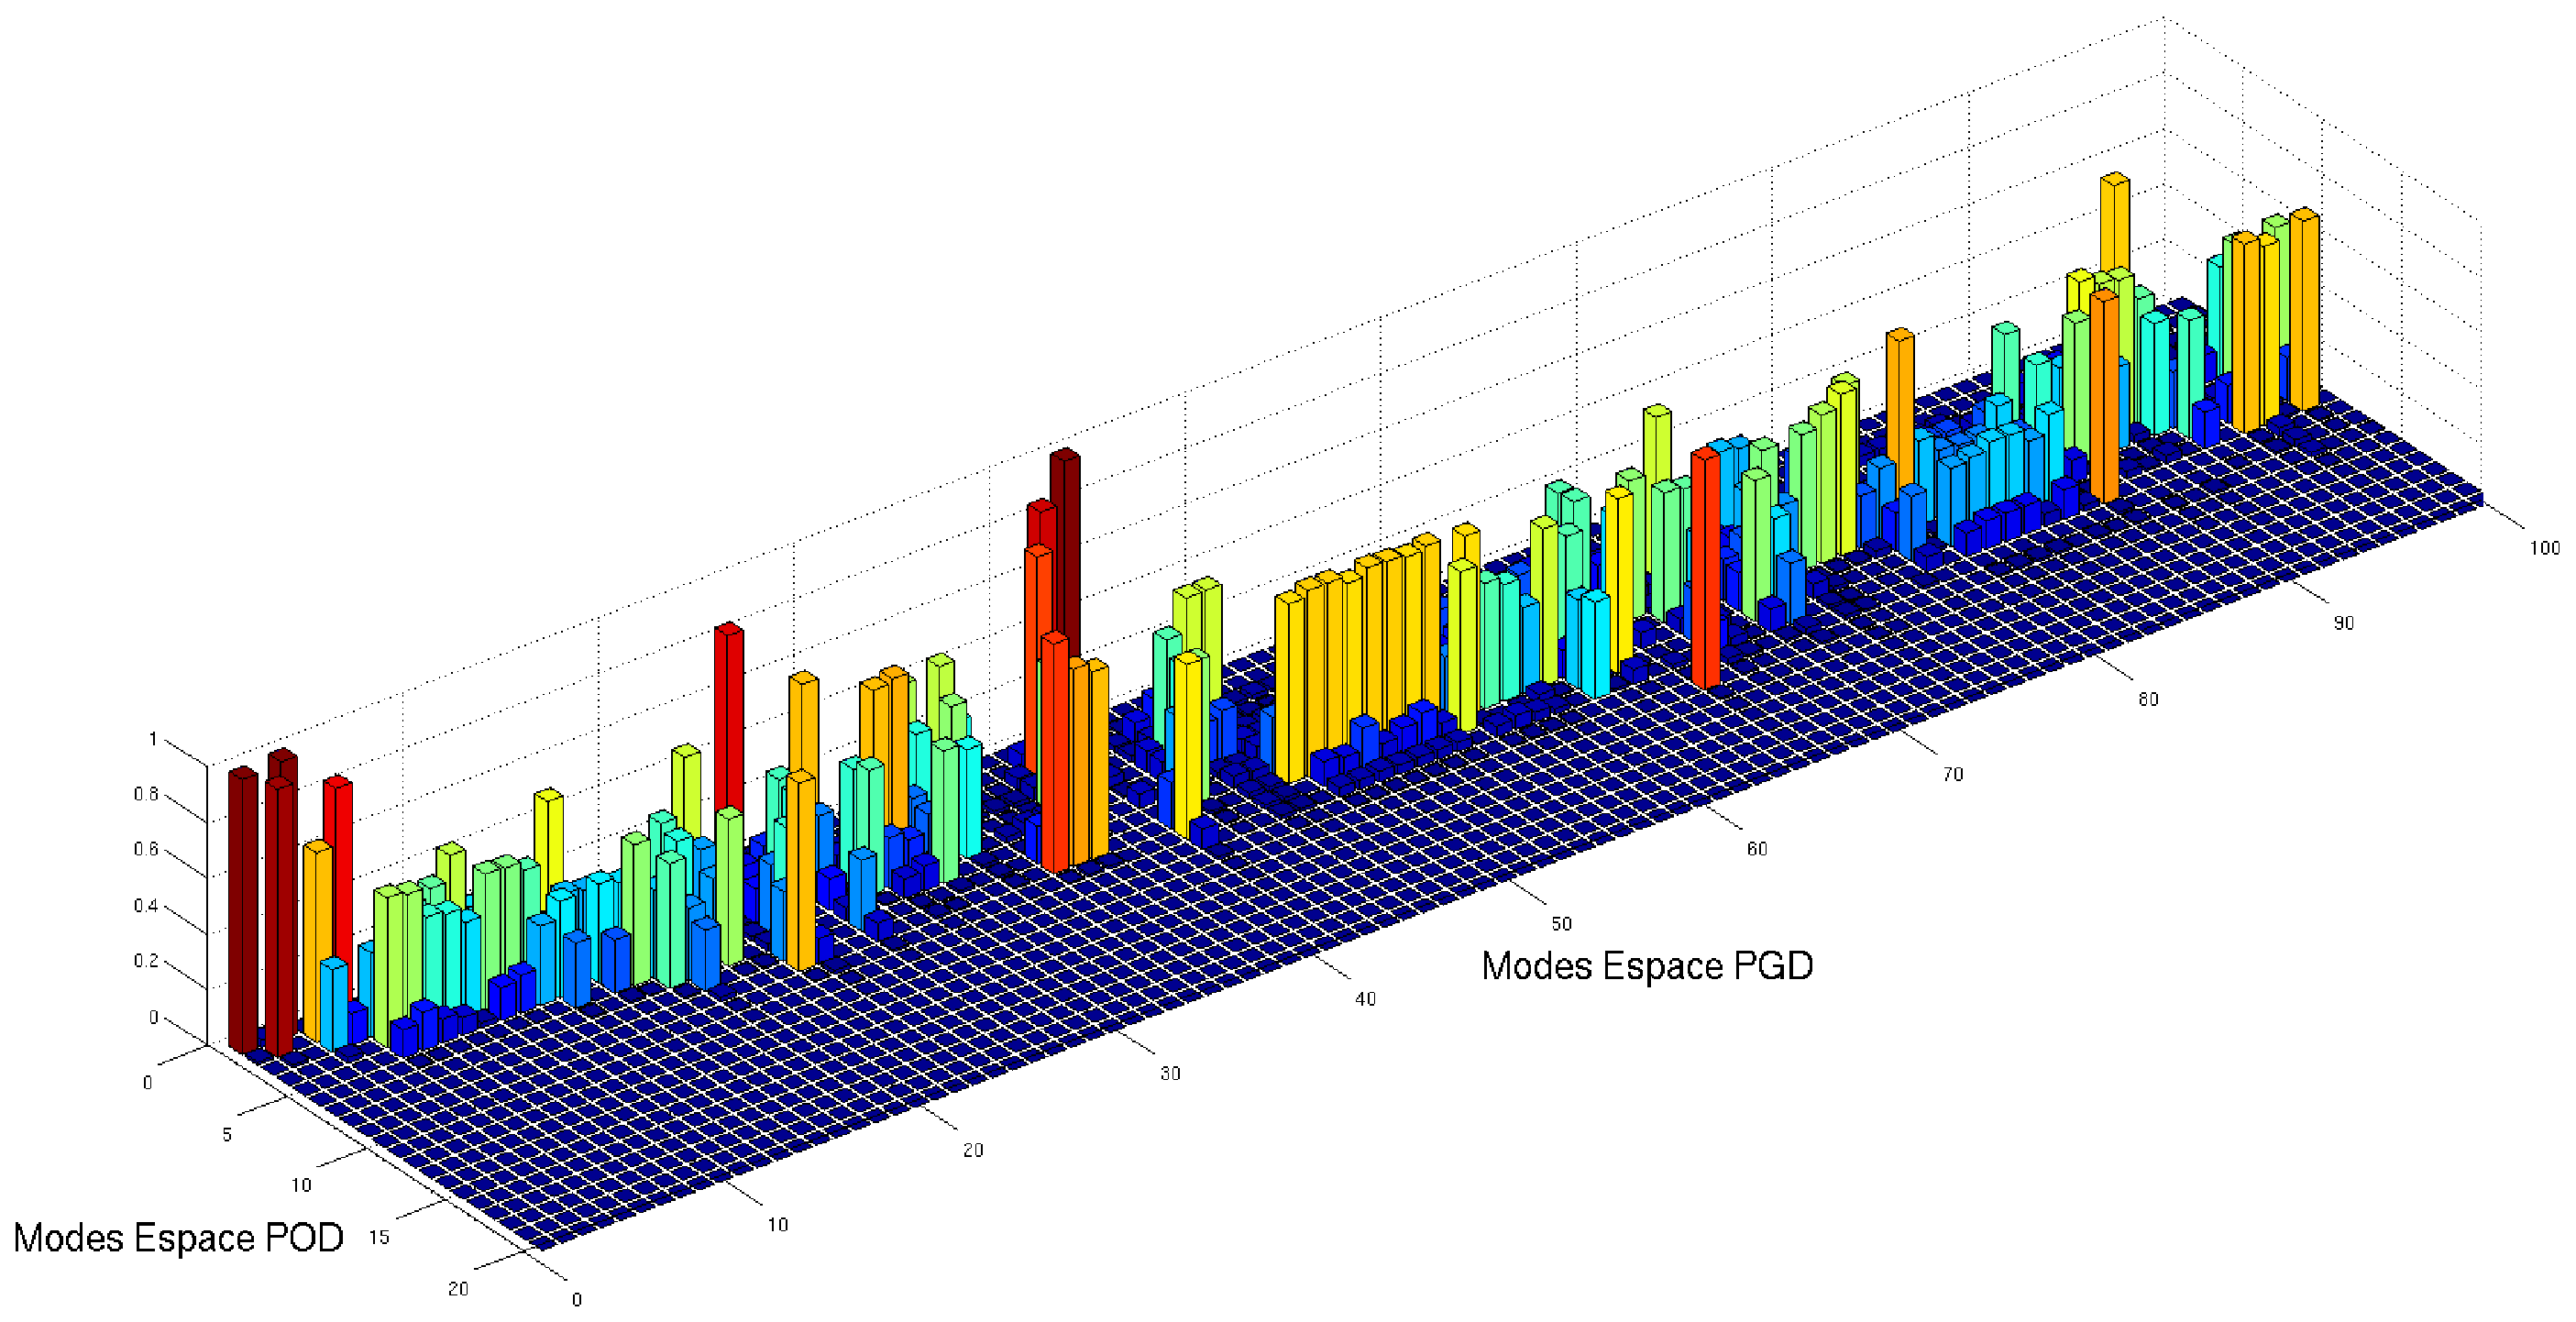
\includegraphics[width=0.9\linewidth]{100ModesAvecNormNonAmortiMAC.eps}
	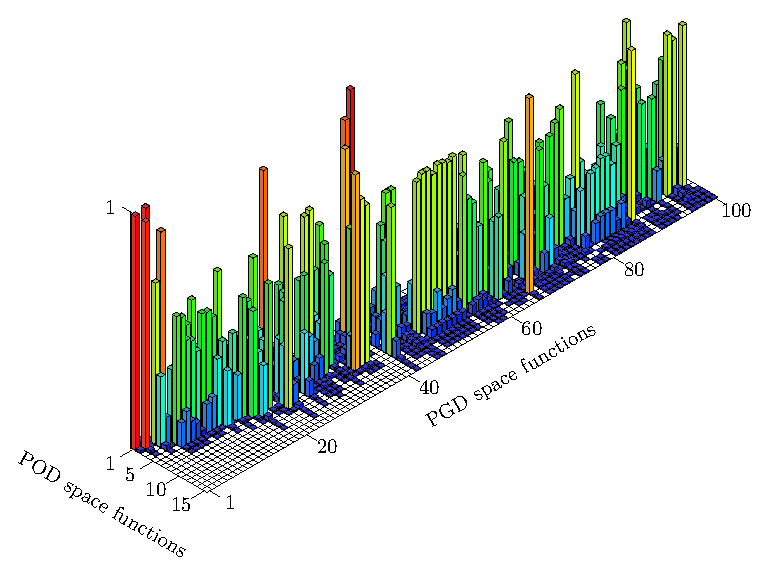
\includegraphics[width=0.7\linewidth]{MAC.POD.PGD.eps}
	\caption{Comparison between POD and PGD space functions}
	\end{figure}
\end{frame}

\subsection{Loading velocity}

\begin{frame}{Loading velocity - Different Cases} 
	\begin{figure}
	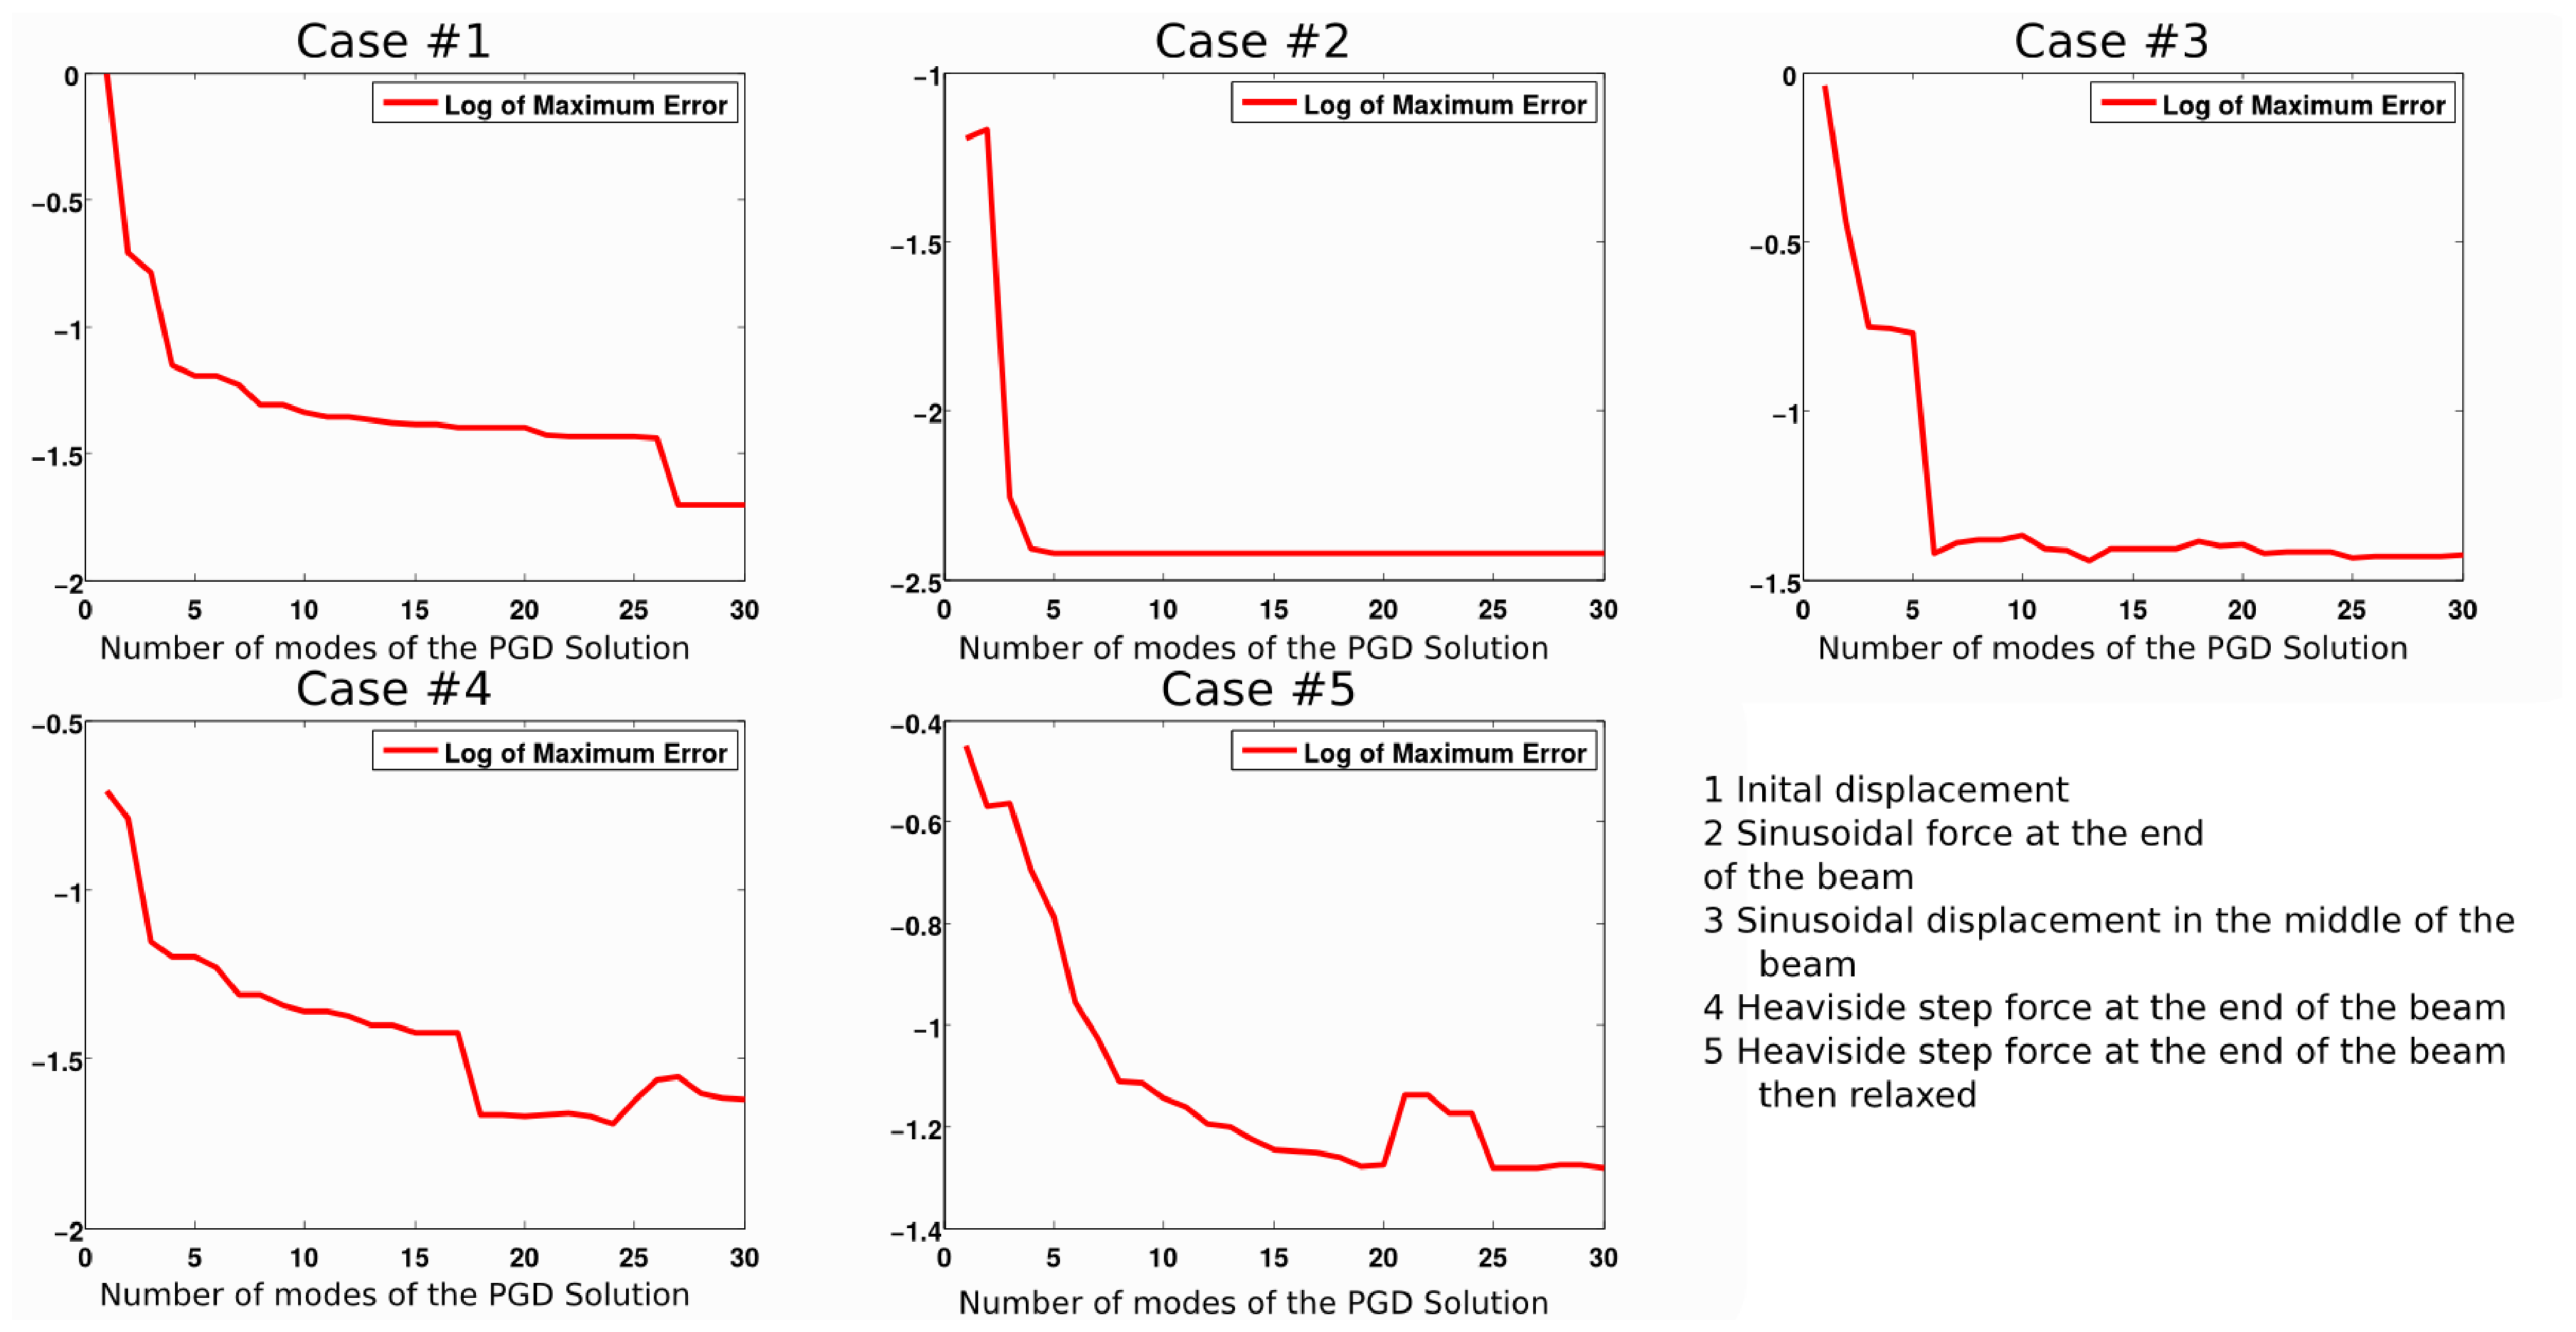
\includegraphics[width=0.98\linewidth]{Cases2.eps}
	\end{figure}
\end{frame}

\begin{frame}{Different Cases - Sinus Verse on a beam} 
	\begin{figure}
		\begin{minipage}[b]{0.4\linewidth}
			\includegraphics[width=1\linewidth]{Beam.tikz.eps}
			\caption{Beam Problem}
		\end{minipage}
		 \hspace{1cm}
		\begin{minipage}[b]{0.4\linewidth}
			\includegraphics[width=1\linewidth]{SinVerse.tikz.eps}
			\caption{Loading}
		\end{minipage}
	\end{figure}
\end{frame}


\begin{frame}{Different Cases - Different Loading Velocities} 
	Loading in Sinus Verse for different period length :
	%Chargement en sinus verse pour différentes rapidités : 
	\begin{figure}
		\begin{minipage}{0.24\linewidth}
			\includegraphics[width=1\linewidth]{CalculSchem3.T4.tikz.eps}
		\end{minipage}
		\begin{minipage}{0.24\linewidth}
			\includegraphics[width=1\linewidth]{CalculSchem3.T3.tikz.eps}
		\end{minipage}
		\begin{minipage}{0.24\linewidth}
			\includegraphics[width=1\linewidth]{CalculSchem3.T2.tikz.eps}
		\end{minipage}
		\begin{minipage}{0.24\linewidth}
			\includegraphics[width=1\linewidth]{CalculSchem3.T1.tikz.eps}
		\end{minipage}
	\end{figure}
	\vspace{-0.4cm}
	
	\begin{figure}
		\begin{minipage}{0.24\linewidth}
			\includegraphics[width=1\linewidth]{Error.CalculSchem3.T4.tikz.eps}
		\end{minipage}
		\begin{minipage}{0.24\linewidth}
			\includegraphics[width=1\linewidth]{Error.CalculSchem3.T3.tikz.eps}
		\end{minipage}
		\begin{minipage}{0.24\linewidth}
			\includegraphics[width=1\linewidth]{Error.CalculSchem3.T2.tikz.eps}
		\end{minipage}
		\begin{minipage}{0.24\linewidth}
			\includegraphics[width=1\linewidth]{Error.CalculSchem3.T1.tikz.eps}
		\end{minipage}
	\end{figure}
\end{frame}

\begin{frame}{Different Time Steps} 
	Violent Case solved with different time steps for the integration scheme :
	%Cas de choc pour différents schémas d'intégration : 
	\begin{figure}
		\begin{minipage}{0.35\linewidth}
			\includegraphics[width=1\linewidth]{CalculSchem3.T1.dt4e-06.tikz.eps}
		\end{minipage}
		 \hspace{1cm}
		\begin{minipage}{0.35\linewidth}
			\includegraphics[width=1\linewidth]{CalculSchem3.T1.dt2e-06.tikz.eps}
		\end{minipage}
	\end{figure}
	\vspace{-0.4cm}
	\begin{figure}
		\begin{minipage}{0.35\linewidth}
			\includegraphics[width=1\linewidth]{CalculSchem3.T1.dt1e-06.tikz.eps}
		\end{minipage}
		 \hspace{1cm}
		\begin{minipage}{0.35\linewidth}
			\includegraphics*[width=1\linewidth]{CalculSchem3.T1.dt5e-07.tikz.eps}
			%\caption{\centering $T=100\times Snapshot$}		
		\end{minipage}
	\end{figure}
\end{frame}

\begin{frame}{Different Integration Schemes} 
	Violent Case solved with different Schemes :
	%Cas de choc pour différents schémas d'intégration : 
	\begin{figure}
		\begin{minipage}{0.35\linewidth}
			\includegraphics[width=1\linewidth]{CalculSchem3b.T1.tikz.eps}
		\end{minipage}
		 \hspace{1cm}
		\begin{minipage}{0.35\linewidth}
			\includegraphics[width=1\linewidth]{CalculSchem4.T1.tikz.eps}
		\end{minipage}
	\end{figure}
	\vspace{-0.4cm}
	\begin{figure}
		\begin{minipage}{0.35\linewidth}
			\includegraphics[width=1\linewidth]{CalculSchem5.T1.tikz.eps}
		\end{minipage}
		 \hspace{1cm}
		\begin{minipage}{0.35\linewidth}
			\includegraphics*[width=1\linewidth]{CalculSchem6.T1.tikz.eps}
			%\caption{\centering $T=100\times Snapshot$}		
		\end{minipage}
	\end{figure}
\end{frame}

\begin{frame}{Time Discontinuous Galerkin Method} 
	\begin{figure}
	\includegraphics[width=0.8\linewidth]{Courbe.Galerkin.DIY.eps}
		\caption{Representation allowing discontinuities}
	\end{figure}
\end{frame}

\section{Perspectives}

\begin{frame}{Perspectives}
	\begin{itemize}
		\item Integration Scheme
			\begin{itemize}
			\item Use of the Galerkin discontinous in time method for the PGD
			\item Influence of the choice of integration scheme on PGD Convergence
			\end{itemize}
		\item Integration in an open FE software
			%\begin{itemize}
			%\item SVD calculation implemented.
			%\end{itemize}
		\item Putting together a work environment for the PGD team
			\begin{itemize}
			\item Adding of parameter variables to the PGD %(Theorical calculation done.)
			\item Using minimization instead of fixed point
			\end{itemize}
		\item Solving non-linear problems
			\begin{itemize}
			\item The usual solver can be used on non-linear problems
			\item Yet to be implemented for the PGD
			\end{itemize}
	\end{itemize}
\end{frame}

\end{document}
